\documentclass{article}
\usepackage[ampersand]{easylist}
\usepackage{amsmath}
\usepackage[inline]{enumitem}
\usepackage{lscape}
\usepackage{graphicx}
\graphicspath{ {C:/Users/ustjo/Desktop/Investing/Stocks/canslim/weeklyStockScanner/Figures/} }
\begin{document}
\title{Weekly Stock Scanner Result \\ 20170925 to 20171001}
\author{KAI YIN, CHAN}
\maketitle

\section{Portfolio}
I have purchased 9 shares of THO at 111.5 with a commission of 0.34 on 2017-09-06, 09:30:02 HKT. The unrealized profit up to September 25, 2017 is 30.06.

\subsection{Action}
\begin{easylist}
& Set sell limit at 129, around 15\% profit.
& Modified stop loss from 105.9 to 109.14, around 5\% loss relative to current stock price as it rises.
\end{easylist}

\section{Stocks that passed scanning}

There are 4 out of 4815 stocks passed the scanning.  They are:
% Table generated by Excel2LaTeX from sheet 'Sheet1'
\begin{table}[htbp]
  \caption{Stocks that passed scanning}
    \begin{tabular}{lllll}
    \textbf{Symbol} & \textbf{Name} & \textbf{Sector} & \textbf{Market Cap} & \textbf{Exchange} \\
    FB    & Facebook, Inc. & Technology & \$495.05B & Nasdaq \\
    KNOP  & KNOT Offshore Partners LP & Consumer Services & \$694.84M & NYSE \\
    NVEE  & NV5 Global, Inc. & Consumer Services & \$556.04M & Nasdaq \\
    THO   & Thor Industries, Inc. & Consumer Non-Durables & \$6.04B & NYSE \\
    \end{tabular}%
  \label{tab:addlabel}%
\end{table}%

\subsection{Actions}
There is a potential buy point of 175.59 for FB as there is a flat base starting on July 31, 2017. (Figure \ref{fig:FBFlatBase})

KNOP does not show good fundamentals after double confirm with online service.

NVEE does not show a potential buy point. 

THO has already broke up from cup with a handle pattern and the price is beyond 5\% buy point.

\begin{figure}[h]
\centering
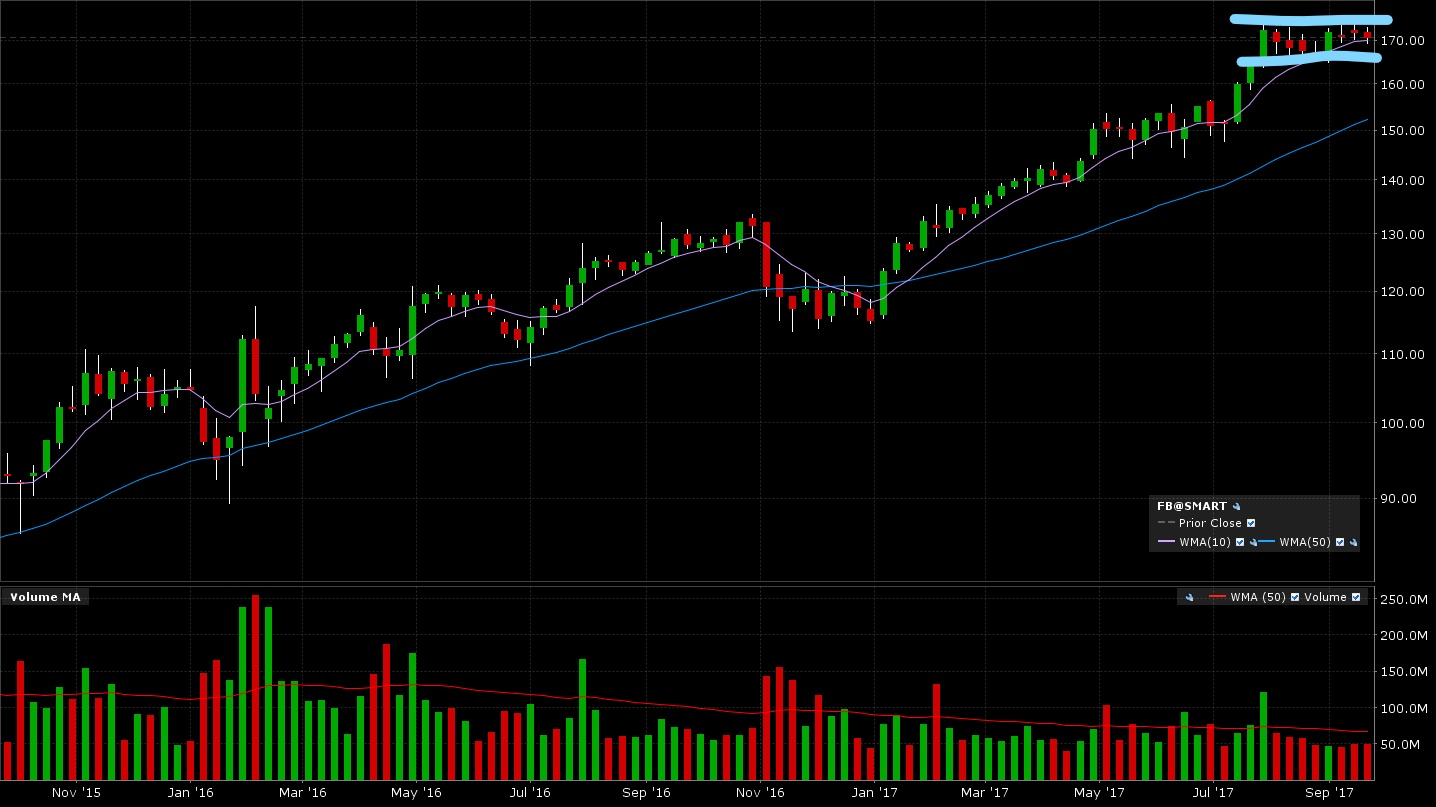
\includegraphics[width=\textwidth]{InkedFBFlatBaseLI_20170925_LI.png}
\caption{FB Flat Base}
\label{fig:FBFlatBase}
\end{figure}

\section{Appendix}
% Table generated by Excel2LaTeX from sheet 'Sheet1'
\begin{table}[htbp]
  \caption{Quarterly EPS}
    \begin{tabular}{lrrrrr}
    \textbf{Symbol} & \multicolumn{1}{l}{\textbf{DEPS Q1}} & \multicolumn{1}{l}{\textbf{DEPS Q2}} & \multicolumn{1}{l}{\textbf{DEPS Q3}} & \multicolumn{1}{l}{\textbf{DEPS Q4}} & \multicolumn{1}{l}{\textbf{DEPS Q5}} \\
    FB    & 1.31955 & 1.04076 & 1.42719 & 0.81612 & 0.78158 \\
    KNOP  & 0.56964 & 0.38816 & 0.71722 & 0.71181 & 0.42576 \\
    NVEE  & 0.40275 & 0.21177 & 0.31282 & 0.32877 & 0.31168 \\
    THO   & 2.10833 & 1.22831 & 1.49404 & 1.5734 & 1.50552 \\
    \end{tabular}%
  \label{tab:addlabel}%
\end{table}%

% Table generated by Excel2LaTeX from sheet 'Sheet1'
\begin{table}[htbp]
  \caption{Quarterly Sales}
    \begin{tabular}{lrrrrr}
    \textbf{Symbol} & \multicolumn{1}{l}{\textbf{TR Q1}} & \multicolumn{1}{l}{\textbf{TR Q2}} & \multicolumn{1}{l}{\textbf{TR Q3}} & \multicolumn{1}{l}{\textbf{TR Q4}} & \multicolumn{1}{l}{\textbf{TR Q5}} \\
    FB    & 9321  & 8032  & 8809  & 7011  & 6436 \\
    KNOP  & 54.406 & 44.992 & 44.995 & 43.587 & 43.063 \\
    NVEE  & 83.736 & 64.059 & 63.022 & 60.091 & 55.892 \\
    THO   & 2015.224 & 1588.525 & 1708.531 & 1292.636 & 1284.054 \\
    \end{tabular}%
  \label{tab:addlabel}%
\end{table}%

% Table generated by Excel2LaTeX from sheet 'Sheet1'
\begin{table}[htbp]
  \caption{EPS, Cash Flow, Sales TTM}
    \begin{tabular}{lrrr}
    \textbf{Symbol} & \multicolumn{1}{l}{\textbf{EPS TTM}} & \multicolumn{1}{l}{\textbf{CashTTM}} & \multicolumn{1}{l}{\textbf{RetTTM}} \\
    FB    & 4.39066 & 5.49475 & 22.04785 \\
    KNOP  & 2.38683 & 4.53658 & 11.4698 \\
    NVEE  & 1.25611 & 2.13505 & 9.02804 \\
    THO   & 6.40408 & 8.14507 & 45.87577 \\
    \end{tabular}%
  \label{tab:addlabel}%
\end{table}%

% Table generated by Excel2LaTeX from sheet 'Sheet1'
\begin{table}[htbp]
  \caption{Annual EPS}
    \begin{tabular}{lrrrrr}
    \textbf{Symbol} & \multicolumn{1}{l}{\textbf{DEPS Y1}} & \multicolumn{1}{l}{\textbf{DEPS Y2}} & \multicolumn{1}{l}{\textbf{DEPS Y3}} & \multicolumn{1}{l}{\textbf{DEPS Y4}} & \multicolumn{1}{l}{\textbf{DEPS Y5}} \\
   FB    & 3.49299 & 1.29267 & 1.1036 & 0.59595 & 0.01477 \\
    KNOP  & 2.24689 & 1.60021 & 1.38504 & 0.87908 &  \\
    NVEE  & 1.21666 & 1.17685 & 0.875 & 0.69548 & 0.52032 \\
    THO   & 4.90625 & 3.79178 & 3.28918 & 2.85559 & 2.06745 \\
    \end{tabular}%
  \label{tab:addlabel}%
\end{table}%

% Table generated by Excel2LaTeX from sheet 'Sheet1'
\begin{table}[htbp]
  \caption{Consensus Earnings and Institutional Ownership}
    \begin{tabular}{lrrrr}
    \textbf{Symbol} & \multicolumn{1}{l}{\textbf{CEPS Y1}} & \multicolumn{1}{l}{\textbf{CEPS Y2}} & \multicolumn{1}{p{4.215em}}{\textbf{Number Institutional Shareholders}} & \multicolumn{1}{p{4.215em}}{\textbf{Institutional Ownership}} \\
    FB    & 5.285 & 6.58  & 3549  & 81 \\
    KNOP  & 2.06  & 2.45  & 107   & 163 \\
    NVEE  & 2.3   & 2.88  & 206   & 88 \\
    THO   & 6.75  & 7.505 & 948   & 134 \\
    \end{tabular}%
  \label{tab:addlabel}%
\end{table}%
\end{document}
